\section{Accessing Participant Data}

On Android, we use the Huawei Health Kit API Java package to request
Huawei Health Kit for the data.
This API allows access to all the collected raw health data points.
We call the API from using Kotlin,
a programming language compatible with Java,
and aggregate the data into a daily summary.
% TODO: What are the data types.
We used Kotlin to integrate with Huawei Health Kit API because
we found it to be more concise and maintainable than Java while
having complete interoperability.
A special pop-up authentication page is also implemented to request the user for
permissions to access their health data, as required by Huawei.

On iOS, we indirectly access Apple HealthKit through Flutter's
Health~\cite{flutterhealth} package.
The Health package provides a unified interface to access health data,
and notifies iOS to request permissions from the user to access the health data.
Since the Health package can also request health data from Google Fit on
Android, we provide an optional feature to use health data from Google Fit to
experimentally accommodate participants who use Android smartphones and
do not use Huawei smartwatches.

In our internal testing, we noticed that accessing the data could be slow,
especially when requesting data using the Huawei Health Kit API.
To mitigate this issue, we implemented a local cache database.
Before we request data from either of the health kits,
we first check the cache database for the data.
If the data is not in the cache database,
we request the data from the health kit and update the cache database.
% TODO: Not implemented yet.
We also implemented a background task to periodically update the cache database,
and the users can also force an update by refreshing the health page in
the application.

\section{The \fedcampus Application}

Most of the \fedcampus Application is implemented in Dart using
the Flutter application framework, with a few exceptions.
The data access on Android and the federated learning on-device training part
calls into platform-specific native code under Flutter's mechanism.

We leverage Flutter's strong support for
building attractive user interface to fulfill the need to
create a user-friendly application.
Additional, HTTP request libraries and JSON libraries in Dart are used to
communicate with the backend,
and an SQL library is used to manage the cache database.

\section{\fedkit}

Overall, \fedkit powers a federated learning system that
consists of a single backend server and a set of mobile application clients.
The clients train their local models on-device with their local data,
and exchange machine learning models and parameters with the backend server to
conduct federated learning.
\fedkit leverages various programming languages and frameworks to achieve its
functionalities, as visualized in Figure~\ref{fig:stack-viz}.

\begin{table}\begin{center}
        \begin{tabular}{llll}\toprule
            Library                   & Functionality                       & Language & Framework       \\\midrule
            Backend Server            & Training Orchestration \& Telemetry & Python   & Django          \\
            Flutter Flower Client     & Backend \& FL Server Communication  & Dart     & Flutter         \\
            TensorFlow Lite Trainer   & Training on Android                 & Kotlin   & TensorFlow Lite \\
            TensorFlow Lite Converter & TensorFlow Models Conversion        & Python   & TensorFlow      \\
            Core ML Trainer           & Training on iOS                     & Swift    & Core ML         \\\bottomrule
        \end{tabular}
        \caption{Major Libraries in the \fedkit Software Development Kit.}
        \label{table:libs}
    \end{center}\end{table}

\fedkit implements 5 libraries, as listed in Table~\ref{table:libs},
to manage client-server communication and simplify on-device machine learning
training.

\begin{figure}\begin{center}
        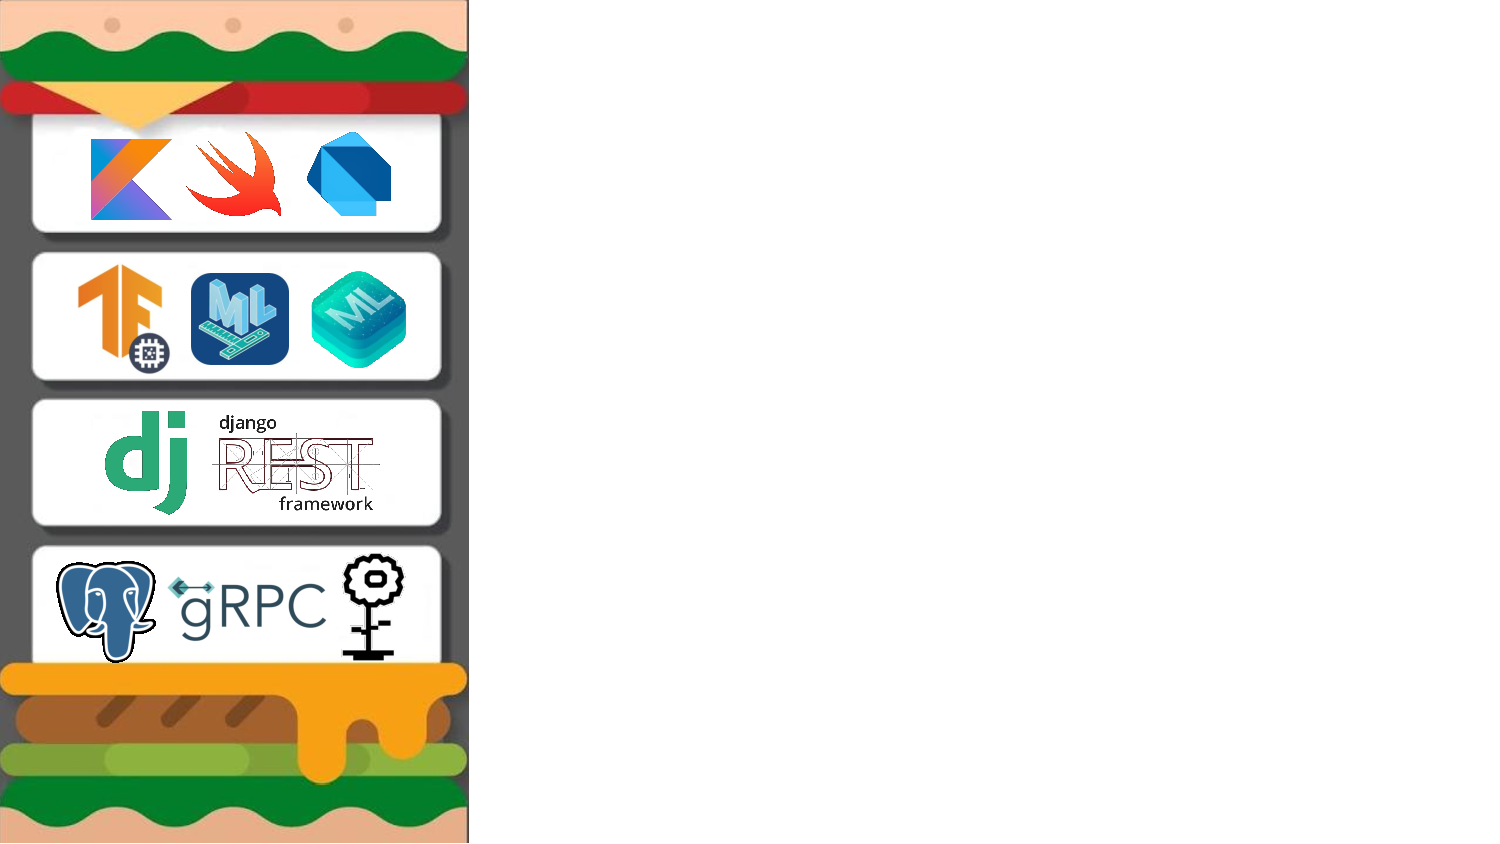
\includegraphics[width=0.4\linewidth]{stack_visualization.pdf}
        \caption{\fedkit Technology Stack Visualization.}
        \label{fig:stack-viz}
    \end{center}\end{figure}

The backend server orchestrates the federated learning process and persists
relevant information in a database through the object-relational mapping the
Django web framework provides. We used SQLite for the database during testing,
and replaced it with PostgreSQL in the deployment. In our deployment,
each model is first uploaded to the backend server,
where model files are stored using the file system and model information is
stored in the database.
Model information is used to determine which clients a model support.
It include whether the model supports TensorFlow Lite or Core ML training,
and a fixed data type that specifies the shape of training input tensors and
labels.
Client applications are bundled with a specific implementation to obtain a
certain data type,
which they use to request the backend server for compatible models.

To reduce the development and maintenance cost operating on both Android and
iOS,
we adopted the Flutter framework to implement the client in our applications to
communicate with the Flower federated learning servers spawned by the backend
server. Since the Flower server leverages gRPC to connect to the clients,
we used the Dart gRPC package to implement the client according to Flower's
protocols.
% TODO: Cite Anthony's Flower Flutter client.
While we intend to record additional telemetry information during training,
we do not want to modify the internals of the Flower servers. Therefore,
we also rely on the Flutter clients to send telemetry information to the backend
server via our representational state transfer application programming
interfaces.
Besides communicating with the backend server and the Flower server,
the Flutter clients also manage the on-device training process by calling into
the platform specific trainers. % TODO: Cite Flutter platform channels.

The TensorFlow Lite Converter is a thin wrapper around TensorFlow to convert
TensorFlow models to the TensorFlow Lite models format we defined in
Section~\ref{sec:pipeline}.
To convert TensorFlow models to Core ML models,
we use the CoreMLTools Python package developed by Apple. After the conversion,
we extract the information about the model layers. For TensorFlow Lite models,
we extract a list of all layers' parameter sizes; for Core ML models,
we extract the layer names, whether they are weights or biases,
and whether they are updatable.
This information is used when aggregating the models and updating the model
parameters on the client, as also discussed in Section~\ref{sec:pipeline}.

While the TensorFlow Lite Trainer directly call the functions defined in the
TensorFlow Lite models, known as ``signatures'',
to complete all federated learning tasks,
the Core ML Trainer additionally uses the Swift ProtoBuf package to inspect and
modify the Core ML model files directly.
% TODO: Cite the Flower Core ML example.
Before training a Core ML model,
we use ProtoBuf to extract all of the model's layers.
To update the model during federated learning,
we use ProtoBuf to manipulate the layer weights and biases in the model file,
and recompile it into a new model,
therefore working around Core ML's artificial prohibition on updating the model
file.
